\chapter{Gesture modeling and recognition}

Compare temporal data modeling: HMM and CRF. 

\section{Temporal Gesture Modeling and Training}

Previous research suggests that
a gesture consists of three phases: \textit{pre-stroke}, \textit{nucleus}, and \textit{post-stroke}~\cite{Pavlovic97}. The pre-stroke phase consists
of a preparatory movement that sets the hand in motion from some resting position.
The nucleus of a gesture has some ``definite form and enhanced dynamic qualities''
~\cite{kendon86}. Finally, the hand either returns to the resting position or repositions
for the new gesture phase. Each gesture
phase includes a sequence of hand/arm movement that can be modeled using HMMs (see Figure~\ref{fig:hmm}). 
This means we can use model temporal gestures as hierarchical hidden Markov
models.

\begin{figure}[h]
\centering
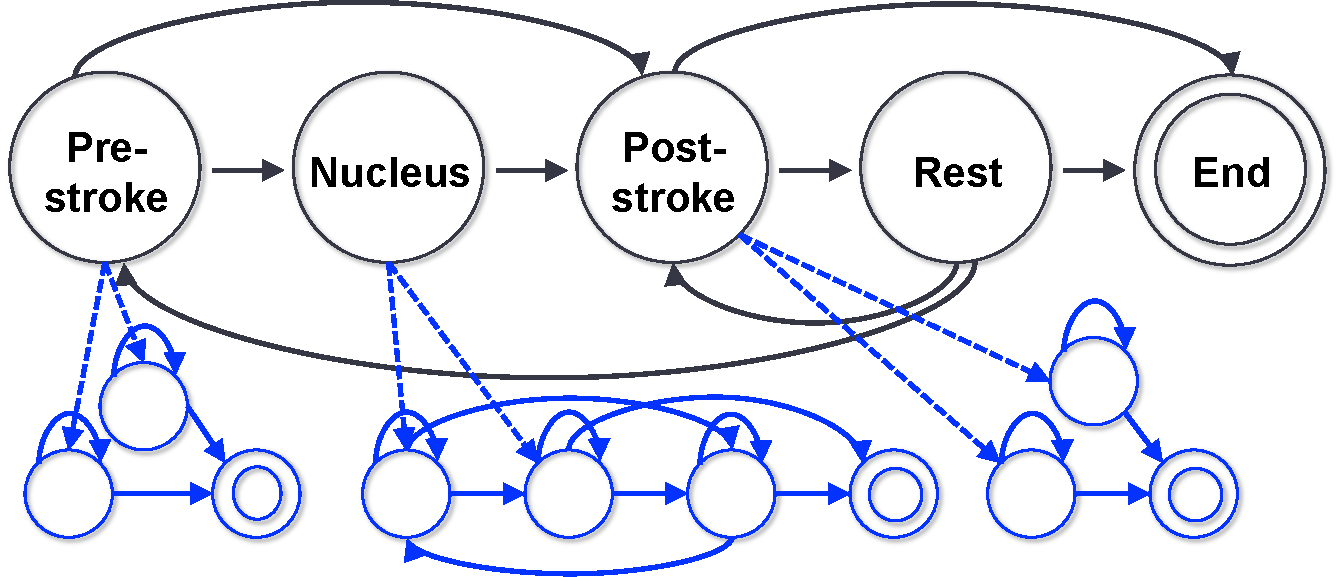
\includegraphics[clip, width=1\columnwidth]{figures/hmm.pdf}
\caption{Temporal gesture model with different phases. Each phase can be modeled as an HMM. Dashed arrows represent
initial state transitions and double circles
represent end states.}
\label{fig:hmm}
\end{figure}

The pre-stroke and post-stroke phases are basically transition phases. We
can also use them to model transitions between different rest positions. We
allow pre-stroke to terminate or go to post-stroke phase. We allow rest state to
go to pre- and post-stroke phases.

Because we have the ground truth labeling of pre-stroke, nucleus and post-stroke phases, 
we can train an HMM for each phase for each gesture. 

\section{Hierarchical Hidden Markov Models}
We combine different levels of recognition using the abstract hidden Markov
model (AHMM) architecture. The AHMM is a probabilistic model used to explain the
interaction between behaviors at different levels of abstraction \cite{johns05}.
It is also closely related to the hierarchical HMM (HHMM) \cite{fine98}. The bottom level in the AHMM 
consists of observations and states in a typical HMM. An HMM is suitable for 
modeling sequential data such as time series, and has been used widely for 
dynamic gesture recognition with reasonable success. We can treat static gesture 
as a special case of dynamic gesture with only one state.

We use a simple 1-level AHMMs \cite{murphy02} (Figure
\ref{fig:amms}). $G_t$ represents the mental concept of the gesture that the
gesturer currently has. It includes unintentional movements ($U$), manipulative
gestures ($M$), and various communicative gestures ($C_i$). $S_t$ is the hidden
state of the hand pose and movement, which is essentially a vector quantization of the actual, observed 
(but noisy) feature vector $X_t$. $F_t^G$ is a binary indicator variable that is
``on'' (has value 1) if the lower level HMM at time $t$ has just ``finished''
(i.e., is about to enter an end state), otherwise it is ``off'' (has value 0).

\tikzstyle{vertex}=[circle, draw, minimum size=16pt, inner sep=0pt]
\tikzstyle{observed-vertex}=[circle, draw, minimum size=16pt, inner sep=0pt,
               fill=black!20] 
\tikzstyle{edge} = [draw, thick, -]
\tikzstyle{directed-edge} = [draw, thick, ->]

\begin{figure}[h]
\centering
  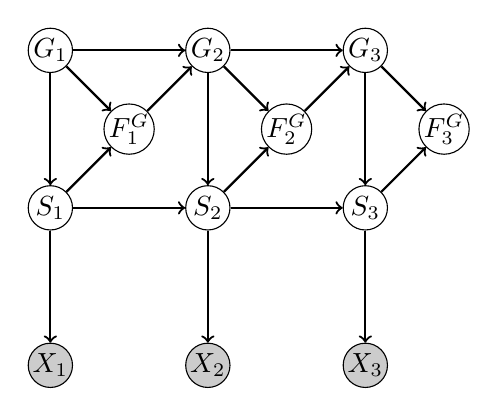
\begin{tikzpicture}[auto,swap, scale=2]
    % First we draw the vertices
    \foreach \pos/\name in {{(0, 2)/G_1}, {(1, 2)/G_2}, {(2,2)/G_3},
      {(0.5,1.5)/F_1^G}, {(1.5,1.5)/F_2^G}, {(2.5, 1.5)/F_3^G},
      {(0, 1)/S_1}, {(1, 1)/S_2}, {(2, 1)/S_3}} 
      \node[vertex] (\name) at \pos {$\name$};
    \foreach \pos/\name in {{(0, 0)/X_1}, {(1, 0)/X_2}, {(2, 0)/X_3}}
      \node[observed-vertex] (\name) at \pos {$\name$};
    % Connect vertices with edges and draw weights
    \foreach \source/ \dest in {G_1/S_1, S_1/X_1, G_1/F_1^G, S_1/F_1^G,
                  F_1^G/G_2, G_1/G_2, G_2/S_2, S_2/X_2, G_2/F_2^G,
                  S_2/F_2^G, F_2^G/G_3, G_2/G_3, G_3/S_3, S_3/X_3,
                  G_3/F_3^G, S_3/F_3^G, S_1/S_2, S_2/S_3} 
      \path[directed-edge] (\source) -- (\dest);
  \end{tikzpicture}
  \caption{A 1-level AHMM. $F_t^G$ turns on if state $S_t$ satisfies goal
  $G_t$; this causes a new goal to be chosen. However, the new state may depend
  on the old state; hence there is no arc from $F_{t-1}^G$ to $S_t$ to
  ``reset'' the submodel \cite{murphy02}.}
  \label{fig:amms}
\end{figure}

\section{Hidden Markov Model}
We use discrete hidden states to represent sub-stages of gestures.

\subsection{Emission Probability}
We use Gaussian emission probability with diagonal covariance. The covariance
has a fixed prior of $0.01\times I$ which is added to the maximum likelihood
estimate to prevent the covariance from shrinking to a point/delta function.

Gaussian mixture, covariance prior 0.01.

\subsection{Termination Probability}
As each phase can have variable length, we model the termination probability for each
hidden state $s$ as $t(\text{END}|s)$. Given a sequence of observation $\underline{X}_1^T = \underline{x}_1\ldots\underline{x}_T$, and 
the corresponding hidden states sequence $S_1^T = s_1\ldots s_T$, we define the probability
\begin{displaymath}
p(\underline{X}_1^T, S_1^T;\underline{\theta}) = 
    t(s_1)t(END|s_T)\prod_{t = 2}^T t(s_t | s_{t-1})\prod_{t = 1}^T e(\underline{x}_t|s_t)
\end{displaymath}
where $\underline{\theta}$ represents the model parameter vector which includes
the initial state probabilities $t(s)$, the state transition probabilities $t(s'|s)$, and the 
emission probabilities $e(\underline{x}|s)$ for $s, s'\in \{1, 2,\ldots k\}$. 
We use a mixture of 6 Gaussians for the emission probability to model user variations.

Given $N$ training sequences, we use the expectation maximization (EM) algorithm to estimate the model parameters. In
particular, the update for the termination probability during the $i$th iteration is 
\begin{displaymath}
t^i(END|s) = \frac{\sum_{j = 1}^N \overline{count}(j, s\rightarrow END;\underline{\theta}^{i-1})}
    {\sum_{j = 1}^N\sum_{s'} \overline{count}(j, s\rightarrow s';\underline{\theta}^{i-1})}
\end{displaymath}
where $\overline{count}(j, s\rightarrow END;\underline{\theta}^{i-1})$ is the expected count of 
$s$ being the end state. We can use the usual forward-backward algorithm to compute all the 
expected sufficient statistics by adding a dummy END state to the end of each sequence.

Because there are 3 rest positions, we use 3 hidden states for both the pre-stroke and post-stroke phases.
Each hidden state can be the start state and can only remain in its own state or go to the end state.
 
For the nucleus phase, we use 6 hidden states (chosen through cross validation) for all the gestures and use a modified Bakis~\cite{bauer2000} model to constrain the transition probabilities
among the hidden states. Instead of allowing only left-right transition, we allow the last hidden state
to go back to the initial state (Figure~\ref{fig:bakis}). This is particularly important for modeling gestures with arbitrary number of
repetitions such as waving and shaking hands. 

When initializing the transition matrix, it is important to make the possible
transitions for each state the same, so that no states are favored arbitrarily.

\subsection{Simple HMM for rest and static hand pose gestures}
One ``rest'' hidden state, transition probability = 1, termination probability =
0.5.

The self-arc on a state in an HMM defines a geometric distribution over waiting
time \cite{murphy02}. Specifically, the probability we remain in state $i$ for
exactly $d$ steps is $p(d) = (1 - p)p^{d - 1}$, where $p = A(i, i)$ is the
self-loop probability. This means the expected number of steps remaining in
state $i$ is $\frac{1}{1 - p}$.

For the rest position, let $t$ be the termination probability of a rest state.
If we assume the minimum duration of rest is 1s (30 frames), 
\begin{align}
\frac{1}{t} > 30 \\
t < \frac{1}{30}
\end{align}

\tikzstyle{vertex}=[circle, draw, minimum size=16pt, inner sep=0pt]
\tikzstyle{observed-vertex}=[circle, draw, minimum size=16pt, inner
sep=0pt, fill=black!20] 
\tikzstyle{edge} = [draw, thick, -]
\tikzstyle{directed-edge} = [draw, ->]

\begin{figure}[tb]
\centering
  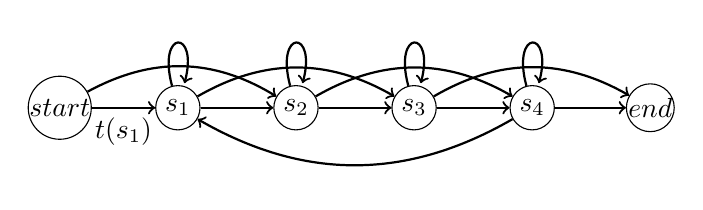
\begin{tikzpicture}[auto,swap, scale=1.5]
    % First we draw the vertices
    \foreach \pos/\name in {{(0, 0)/start}, {(1, 0)/s_1}, {(2, 0)/s_2},
    {(3, 0)/s_3}, {(4, 0)/s_4}, {(5, 0)/end}}
      \node[vertex] (\name) at \pos {$\name$};
    % Connect vertices with edges and draw weights
    \foreach \source/ \dest in {s_2/s_3, s_3/s_4, s_4/end,
    s_1/s_2} \path[directed-edge] (\source) -- (\dest);
    
    \foreach \source/ \dest in {s_1/s_3, start/s_2, s_2/s_4, s_3/end, s_4/s_1} 
      \path[directed-edge] (\source) edge [bend left] (\dest);
      
    \foreach \source/ \dest in {s_1/s_1, s_2/s_2, s_3/s_3, s_4/s_4} 
      \path[directed-edge] (\source) edge [loop above] (\dest);
    
    \path[directed-edge] (start) edge node [below] {$t(s_1)$} (s_1);
  \end{tikzpicture}
  \caption{A state transition diagram of a modified 4-state Bakis model for the nucleus phase.}
  \label{fig:bakis}
\end{figure}

\subsection{Gesture Recognition}
During the recognition phase, we concatenate the HMMs trained for each phase together to form
one HMM for each gesture. The transition probability from the previous phase to the next
phase can be computed by multiplying the termination probabilities of the previous phase and the
initial state probabilities of the next phase. Using the superscript $c$ to denote the model
parameters in the concatenated HMM, we have
\begin{displaymath}
t^c(s_\text{nucleus}|s_\text{prestroke}) = t(\text{END}|s_\text{prestroke}) \times t(s_\text{nucleus})
\end{displaymath}
where $s_{\text{phase}}$ denotes the hidden state variable in a particular phase. We add small transition
probabilities from the pre-stroke phase to the post-stroke phase to model movements that do not have the 
nucleus phase.

As new state transition probabilities are added, the transition probabilities among
states in the same phase also need to be modified so that $\sum_{s' = 1}^K t(s'|s) = 1$ (where
$K$ is the total number of combined hidden states) is ensured. For example
\begin{displaymath}
t^c(s'_{\text{nucleus}} | s_{\text{nucleus}}) = t(s'_{\text{nucleus}} | s_{\text{nucleus}})
  \times (1 - t(\text{END} | s_{\text{nucleus}}))
\end{displaymath}

We also add a rest state to the end of the HMM and allow the rest state to transit to the pre-stroke
and the post-stroke phase with uniform probabilities (Figure~\ref{fig:hmm}) to accommodate short pauses during the gesture.
As a result, the final HMM for each gesture has 13 hidden states.
Let $\underline{\theta}_g$ be the final concatenated HMM parameters for gesture $g$. The classification
of an observation sequence from non-rest positions is 
\begin{displaymath}
\hat{g} = \arg\max_g\log p(\underline{X}_1^T; \underline{\theta}_g)
\end{displaymath}

\subsection{Gesture Spotting}
Because the non-rest positions include both pre-stroke and post-stroke phases, we need
to detect the start of the actual gesture (nucleus). We use the Viterbi algorithm
to find the most probable hidden state sequence $\hat{s}_1\ldots\hat{s}_T$ for a given observed sequence using 
the mostly likely gesture model $\underline{\theta}_{\hat{g}}$. The start and the end time for a gesture nucleus are
the first and the last time frame $t$ where $\hat{s}_t\in s_{\text{nucleus}}$ respectively. Note that
we are able to identify whether a hidden state belongs to the nucleus phase because we trained the three phases
separately.

\begin{figure}[tb]
\centering
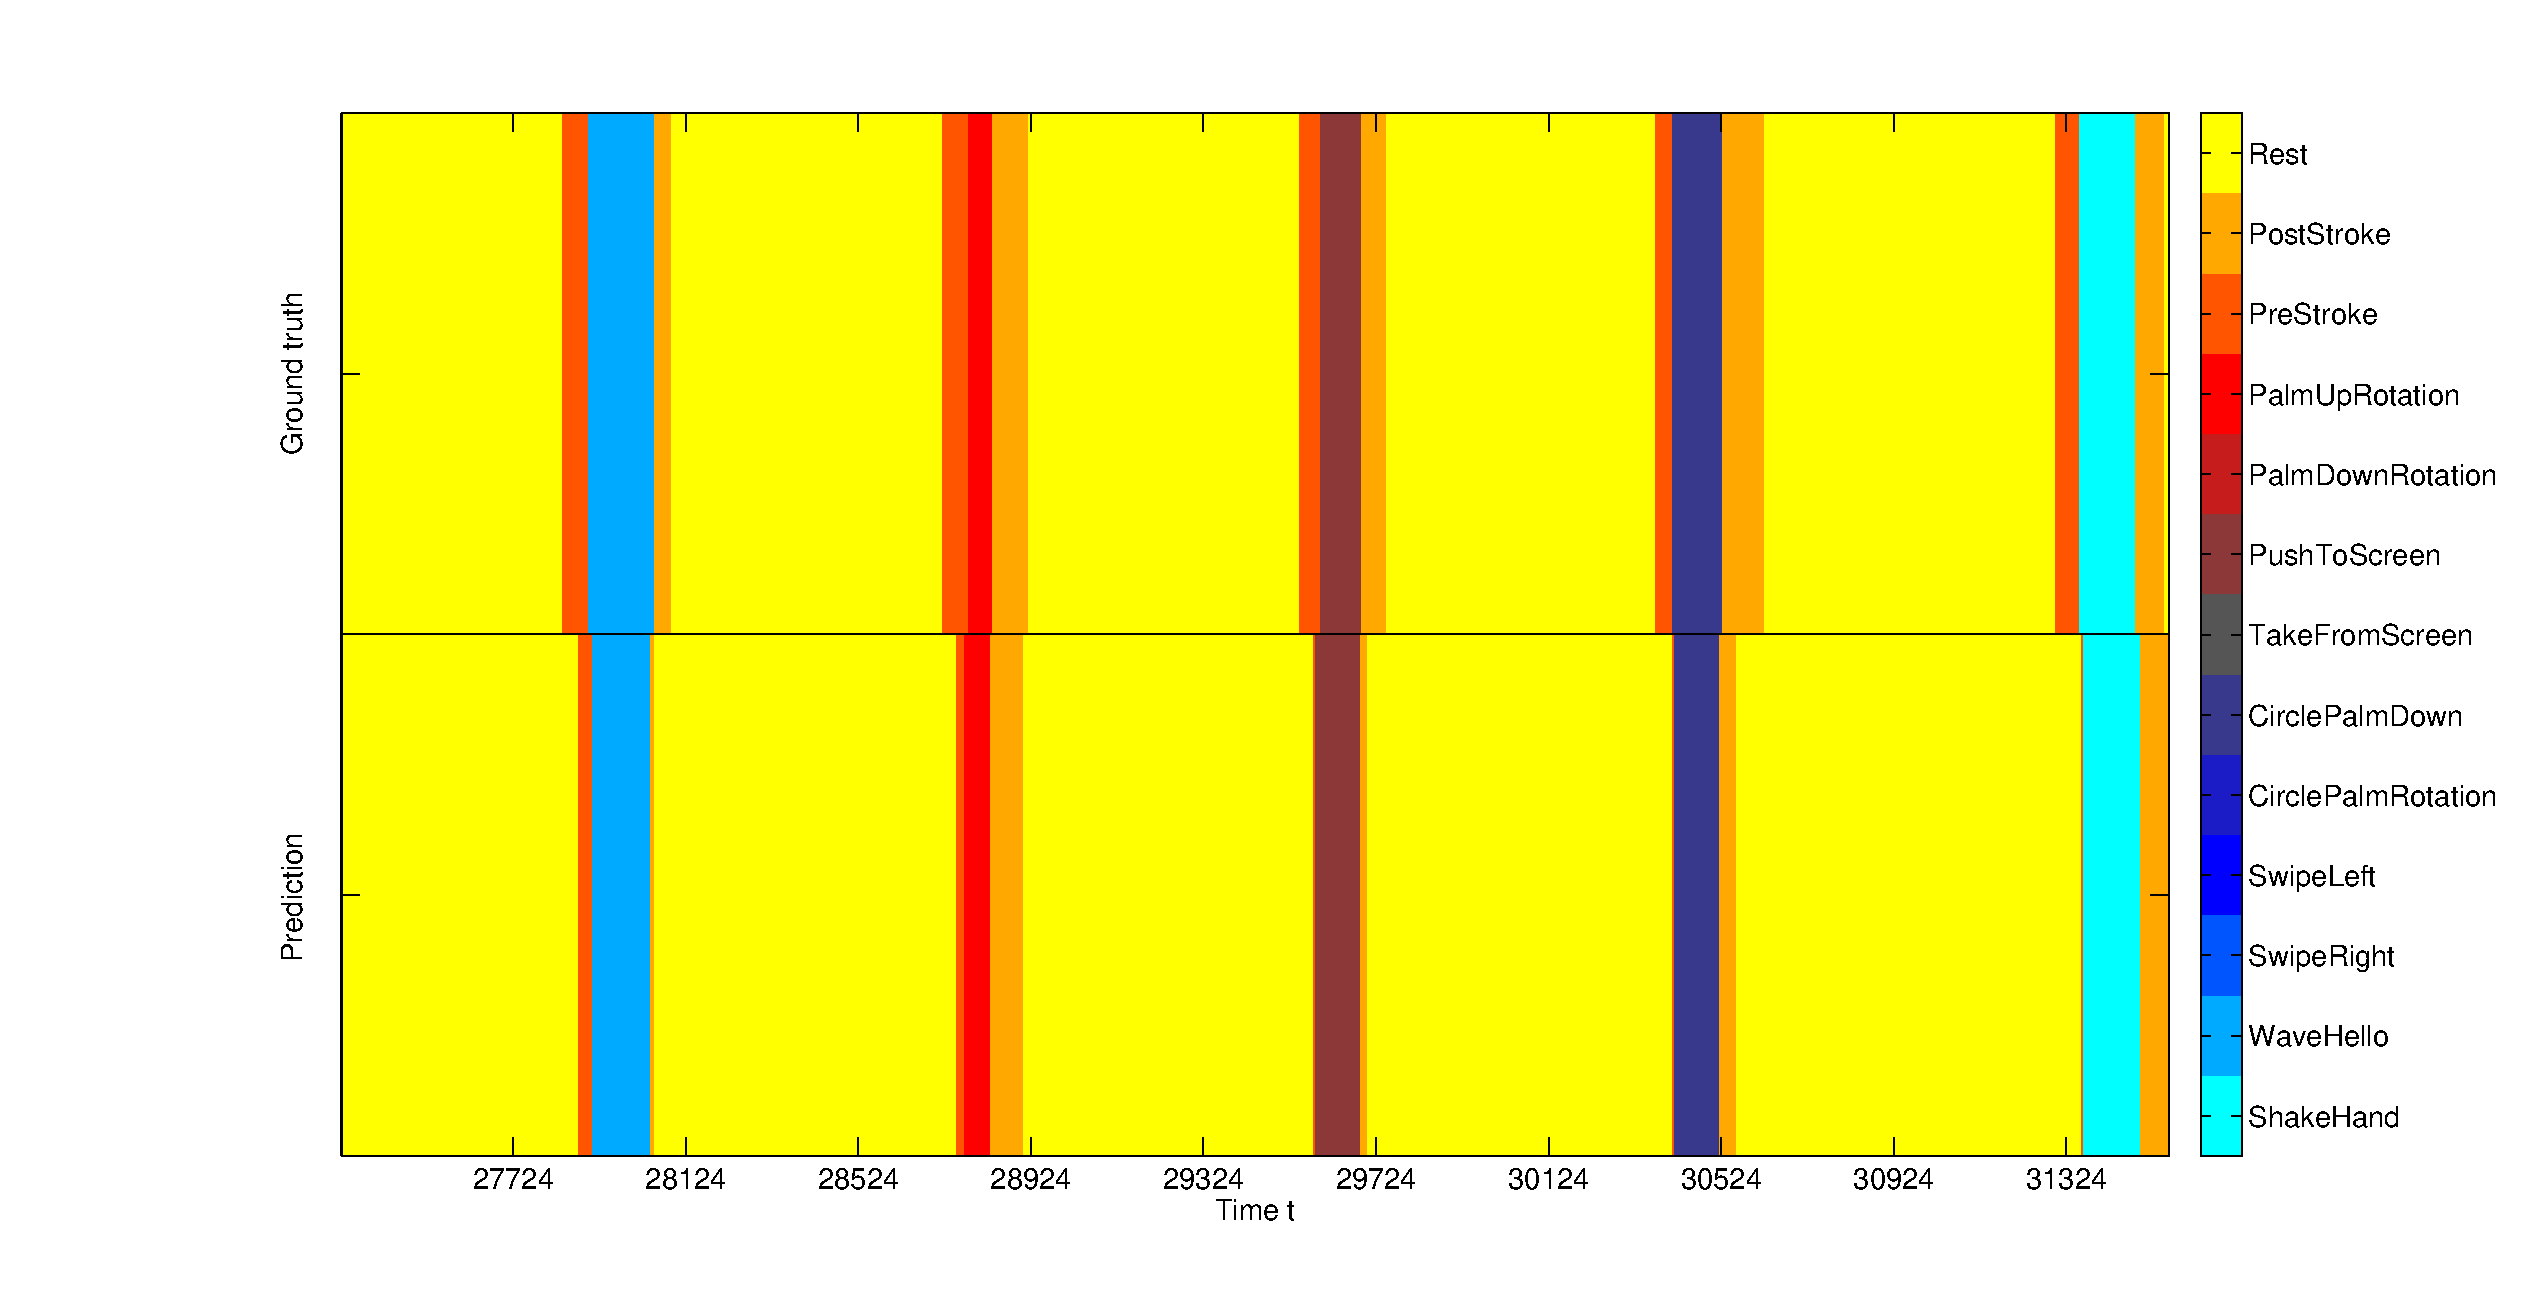
\includegraphics[trim={4cm 1cm 0cm 0.6cm}, clip,
width=1\columnwidth]{figures/gesture.eps} \caption{Visualization of a gesture
recognition sequence.
The pre-stroke and post-stroke phases are indicated by two orange colors (see the color bar).}
\label{fig:decoding}
\end{figure}

\begin{figure}[tb]
\centering
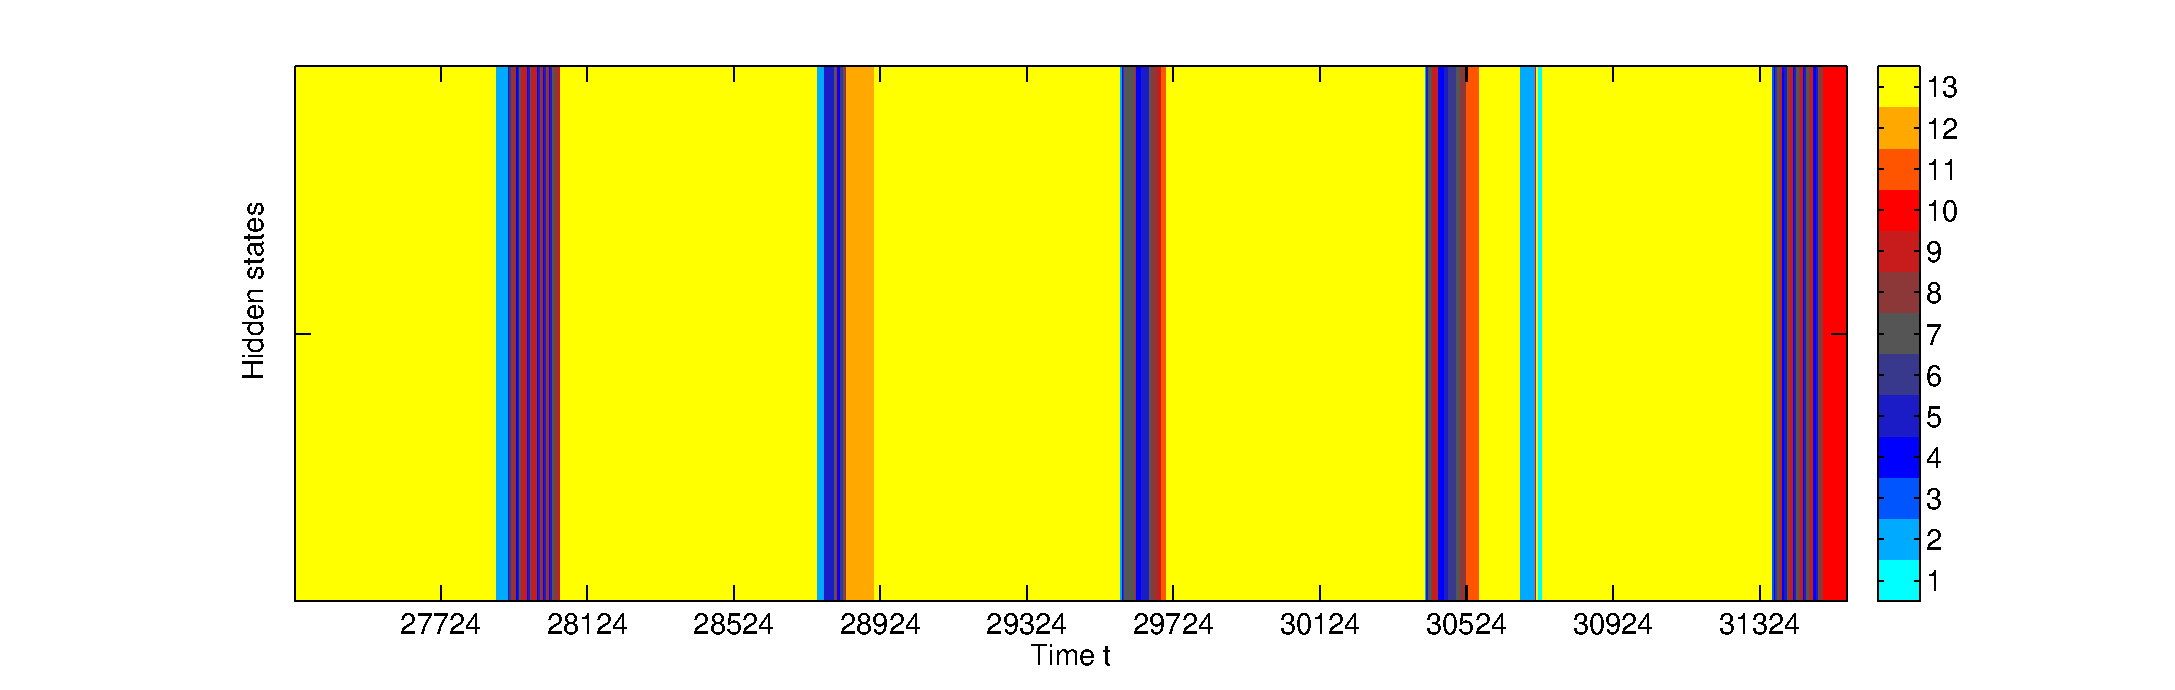
\includegraphics[trim={3.5cm 0cm 0.5cm 0cm}, clip,
width=1\columnwidth]{figures/hiddenstates.eps} \caption{Visualization of the
most probable hidden states of a gesture recognition sequence.
Colors 1-3 indicate the pre-stroke hidden states, colors 4 - 9
indicate the nucleus hidden states, colors 10 - 12 indicate the post-stroke
hidden states, and color 14 indicates the rest state.}
\label{fig:hiddenstates}
\end{figure}

Figure~\ref{fig:decoding} shows a recognition result visualization for one batch sequence. The first
row is the ground truth with different colors indicating different gesture phases or the rest position. 
The second row is our segmentation and recognition result.
Figure~\ref{fig:hiddenstates} shows the color-coded most probable hidden states
for the same sequence.
If a non-rest sequence does not contain hidden states belonging to the nucleus
phase, it is ignored (see the blue bar at $t\sim 30700$ in Figure~\ref{fig:hiddenstates}).
In this way, we can spot the actual gestures while filtering out other movements.

\section{Conditional Random Field}

\section{Online Inference}
On Chairgest data.